\documentclass[a4paper,12pt, oneside]{book}

% \usepackage{fullpage}
\usepackage[italian]{babel}
\usepackage[utf8]{inputenc}
\usepackage{amssymb}
\usepackage{amsthm}
\usepackage{graphics}
\usepackage{amsfonts}
\usepackage{listings}
\usepackage{amsmath}
\usepackage{amstext}
\usepackage{engrec}
\usepackage{rotating}
\usepackage{verbatim}
\usepackage[safe,extra]{tipa}
% \usepackage{showkeys}
\usepackage{multirow}
\usepackage{hyperref}
\usepackage{microtype}
\usepackage{fontspec}
\usepackage{enumerate}
\usepackage{physics}
\usepackage{braket}
\usepackage{marginnote}
\usepackage{pgfplots}
\usepackage{cancel}
\usepackage{polynom}
\usepackage{booktabs}
\usepackage{enumitem}
\usepackage{framed}
\usepackage{pdfpages}
\usepackage{pgfplots}
\usepackage{algorithm}
% \usepackage{algpseudocode}
\usepackage[cache=false]{minted}
\usepackage{mathtools}
\usepackage[noend]{algpseudocode}
\newcommand*{\bfrac}[2]{\genfrac{}{}{0pt}{}{#1}{#2}}

\usepackage{tikz}\usetikzlibrary{er}\tikzset{multi  attribute /.style={attribute
    ,double  distance =1.5pt}}\tikzset{derived  attribute /.style={attribute
    ,dashed}}\tikzset{total /.style={double  distance =1.5pt}}\tikzset{every
  entity /.style={draw=orange , fill=orange!20}}\tikzset{every  attribute
  /.style={draw=MediumPurple1, fill=MediumPurple1!20}}\tikzset{every
  relationship /.style={draw=Chartreuse2,
    fill=Chartreuse2!20}}\newcommand{\key}[1]{\underline{#1}}
\usetikzlibrary{arrows.meta}
\usetikzlibrary{decorations.markings}
\usetikzlibrary{arrows,shapes,backgrounds,petri}
\tikzset{
  place/.style={
    circle,
    thick,
    draw=black,
    minimum size=6mm,
  },
  transition/.style={
    rectangle,
    thick,
    fill=black,
    minimum width=8mm,
    inner ysep=2pt
  },
  transitionv/.style={
    rectangle,
    thick,
    fill=black,
    minimum height=8mm,
    inner xsep=2pt
  }
} 
\usetikzlibrary{automata,positioning,chains,fit,shapes}
\usepackage{fancyhdr}
\pagestyle{fancy}
\fancyhead[LE,RO]{\slshape \rightmark}
\fancyhead[LO,RE]{\slshape \leftmark}
\fancyfoot[C]{\thepage}
\usepackage[usenames,dvipsnames]{pstricks}
\usepackage{epsfig}
\usepackage{pst-grad} % For gradients
\usepackage{pst-plot} % For axes
\usepackage[space]{grffile} % For spaces in paths
\usepackage{etoolbox} % For spaces in paths
\makeatletter % For spaces in paths
\patchcmd\Gread@eps{\@inputcheck#1 }{\@inputcheck"#1"\relax}{}{}
\makeatother
\usepackage{lipsum}
\DeclareSymbolFont{symbolsC}{U}{txsyc}{m}{n}
\DeclareMathSymbol{\strictif}{\mathrel}{symbolsC}{74}
\title{Computational Systems Biology}
\author{UniShare\\\\Davide Cozzi\\\href{https://t.me/dlcgold}{@dlcgold}}
\date{}

\pgfplotsset{compat=1.13}
\begin{document}
\maketitle

\definecolor{shadecolor}{gray}{0.80}
\setlist{leftmargin = 2cm}
\newtheorem{teorema}{Teorema}
\newtheorem{definizione}{Definizione}
\newtheorem{esempio}{Esempio}
\newtheorem{corollario}{Corollario}
\newtheorem{lemma}{Lemma}
\newtheorem{osservazione}{Osservazione}
\newtheorem{nota}{Nota}
\newtheorem{esercizio}{Esercizio}
\algdef{SE}[DOWHILE]{Do}{doWhile}{\algorithmicdo}[1]{\algorithmicwhile\ #1}
\tableofcontents
\renewcommand{\chaptermark}[1]{%
  \markboth{\chaptername
    \ \thechapter.\ #1}{}}
\renewcommand{\sectionmark}[1]{\markright{\thesection.\ #1}}
\newcommand{\floor}[1]{\lfloor #1 \rfloor}
\newcommand{\MYhref}[3][blue]{\href{#2}{\color{#1}{#3}}}%
\chapter{Introduzione}
\textbf{Questi appunti sono presi a lezione. Per quanto sia stata fatta
  una revisione è altamente probabile (praticamente certo) che possano
  contenere errori, sia di stampa che di vero e proprio contenuto. Per
  eventuali proposte di correzione effettuare una pull request. Link: }
\url{https://github.com/dlcgold/Appunti}.\\
\chapter{Introduzione alla Systems Biology}
Per descrivere sistemi biologici complessi si hanno vari tipi di modelli.\\
Kitano (il ``padre'' di quest'ambito), nel 2002, disse che per capire i sistemi
biologici complessi bisogna integrare risultati sperimentali e metodi
computazionali, ottenendo quindi la 
vera e propria \textbf{Systems Biology}. Tramite l'interazione di vari
componenti si ottengono tali sistemi. Disse infatti:
\begin{center}
  \textit{To understand complex biological systems requires the integration of
    experimental and computational research — in other words a systems biology
    approach.} 
\end{center}
Weston, nel 2004, ha aggiunto l'importanza dello studio delle interazioni e
delle regolazioni tra i vari componenti del sistema, studiando le risposte alla
genetica o alle perturbazioni ambientali, al fine di capire nuove proprietà del
sistema. Infatti disse:
\begin{center}
  \textit{Systems biology is the analysis of the relationships among the
    elements in a system in response to genetic or environmental perturbations,
    with the goal of understanding the system or the emergent properties of the
    system} 
\end{center}
Ideker (altro ``padre'' di quest'ambito), già nel 2001, aveva definito la System
Biology come l'integrazione dei 
dati sperimentali con i modelli matematici che descrivono componenti e
interazioni, al fine di simulare il comportamento complessivo ``in silico''. Nel
dettaglio, citandolo:
\begin{center}
  \textit{Systems biology studies biological systems by systematically
    perturbing them (biologically, genetically, or chemically); monitoring the
    gene, protein, and informational pathway responses; integrating these data;
    and ultimately, formulating mathematical models that describe the structure
    of the system and its response to individual perturbations} 
\end{center}
Ai metodi standard della biologia quindi si aggiungono le teorie
informatiche, quelle matematiche, quelle fisiche, quelle chimiche, quelle
ingegneristiche. A partire dal fenomeno biologico quindi si effettuando
esperimenti, ottenendo dei dati sperimentali relativi alle funzioni, alle
strutture e alle interazioni delle varie componenti biologiche. A partire da
questi dati si costruisce un \textbf{modello matematico} che porterà alla
produzione 
di \textit{ipotesi} a partire da esso. Inoltre l'insieme di ipotesi produrrà
nuovi dati che potranno essere anche usati per rifinire il modello
stesso. Inoltre tali ipotesi possono portare a sperimentazioni in \textbf{dry
  lab}, quindi ``in silico'' tramite simulazioni, ma anche in \textbf{wet lab},
quindi in laboratorio qualora possibile. Tali sperimentazioni contribuiranno a
migliorare i dati stessi, producendone anche di nuovi. Si ha quindi un sistema
ciclico di costante miglioramento della ricerca stessa, come visualizzabile in
figura \ref{fig:csb}.\\
\begin{figure}
  \centering
  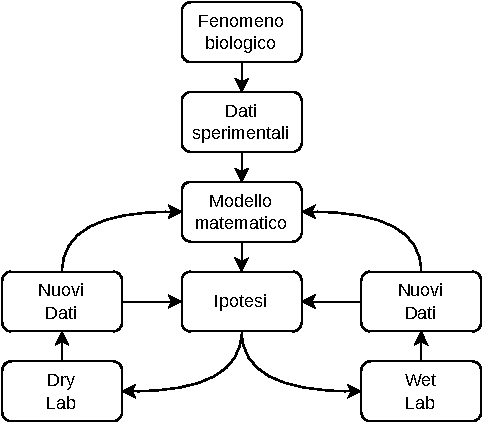
\includegraphics[scale = 0.8]{img/csb.pdf}
  \caption{Grafico rappresentante il processo ciclico della Systems Biology.} 
  \label{fig:csb}
\end{figure}
Un altro aspetto fondamentale del discorso è capire cosa \textbf{non} sia la
\textit{systems biology}. Citando Wolkenhauer \footnote{O. Wolkenhauer, Why
  Systems Biology is (not) called Systems Biology, BIOforum Europe 4/2007}:
\begin{center}
  \textit{Opening then the book, which I discovered in the London bookstore, I
    read the contents list: “Shotgun Fragment Assembly”, “Gene Finding”, “Local
    Sequence Similarities”, ... What?? ... “Protein Structure Prediction”, “Some 
    Computational Problems Associated with Horizontal Gene Transfer” ... what on
    earth has this to do with systems biology, I asked myself?}\\
  \textit{...}\\
  \textit{Most important to me is
    however that cells and proteins are in  teracting in space and time, that
    is, we are dealing here with (nonlinear) dynamic systems. If you ask me
    then, systems biology is a merger of systems theory with cell biology.}
  \\
  \textit{...}\\
  \textit{Systems biology and bioinformatics are different but complementary.}
\end{center}
Infatti tematiche come l'assemblaggio, l'allineamento etc$\ldots$ non sono
tematiche della \textit{systems biolog}y ma della \textit{bioinformatica},
nonostante spesso vengano confuse e sovrapposte. L'analisi diretta dei dati
biologici non è campo della \textit{systems biology} in quanto si perde uno
degli aspetti fondamentali, ovvero quello del \textbf{tempo}, che comporta lo
studio di \textbf{sistemi dinamici}, che appunto di evolvono nel tempo. In
bioinformatica d'altro canto si ha spesso a che fare con dati provenienti da
pochi timestamp (se non direttamente da uno solo). Inoltre, sempre in
bioinformatica, si studiano solitamente poche componenti biologiche, senza
studiarne l'interazione tra esse.\\
La domanda più importante della \textit{systems biology}, della quale possiamo
vedere uno schema generale delle fasi in figura \ref{fig:csb2}, è quindi:
\begin{center}
  \textit{dato un sistema biologico d'interesse, di cui si vogliono studiare le
    funzioni etc$\ldots$, quale approccio modellistico è più adatto per
    descrivere quel sistema?}
\end{center}
Una volta risposto a questo quesito bisogna ovviamente capire quale sia lo
strumento computazionale di cui si ha bisogno per simulare e analizzare tale
sistema. Bisogna infine capire quali predizioni si possono ottenere da questo
modello, che comunque deve prima essere validato. Tra le cose principali che si
vogliono capire abbiamo, ad esempio, se si può controllare il sistema e se si
può riprodurre il tutto in laboratorio riducendo il numero di tentativi e di
conseguenza anche il costo dell'esperimento in \textit{wet lab}.\\
\begin{figure}
  \centering
  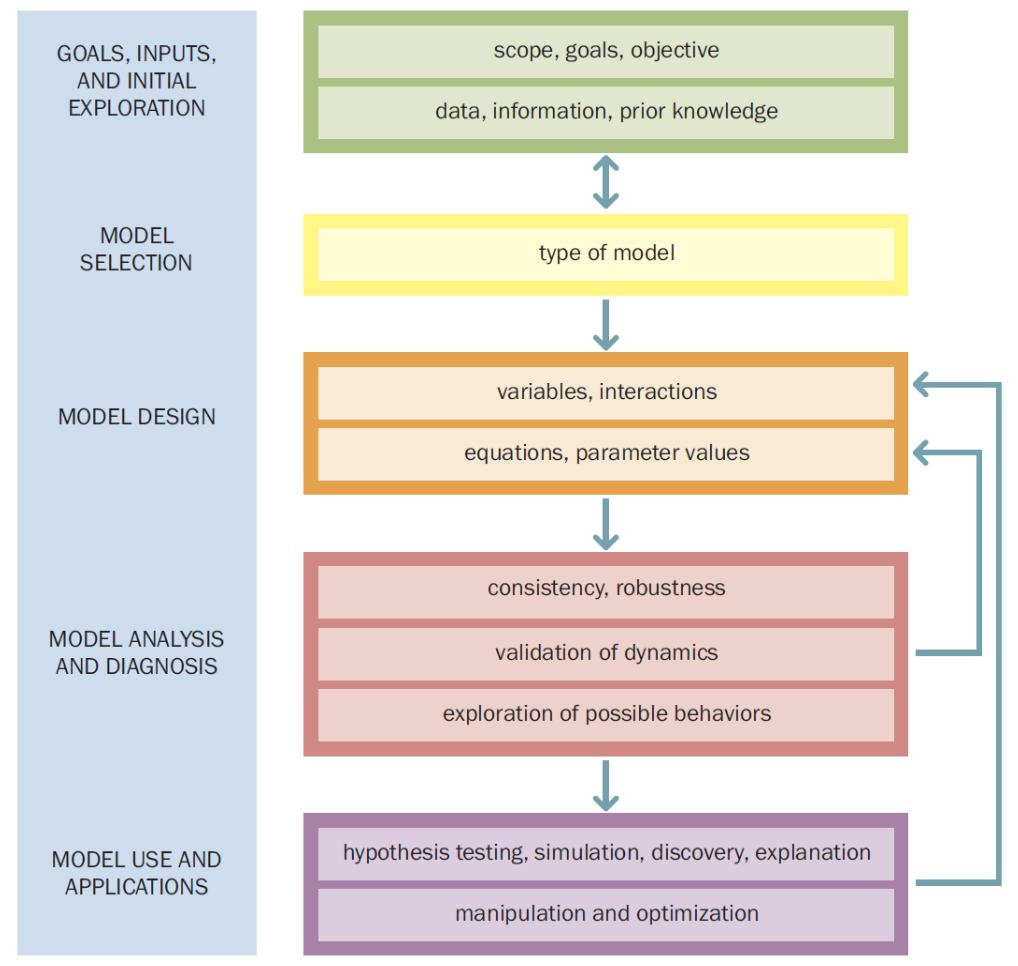
\includegraphics[scale = 0.3]{img/csb2.jpg}
  \caption{Schema generale delle fasi tipiche che compongono la systems
    biology.} 
  \label{fig:csb2}
\end{figure}
Possiamo quindi facilmente intuire che uno degli aspetti fondamentali di questo
ambito è quello di fare le corrette \textit{assunzioni}. Citando ancora
Wolkenhauer \footnote{O. Wolkenhauer, Why Systems Biology is (not) called
  Systems Biology, BIOforum Europe 4/2007}:
\begin{center}
  \textit{The modelling process itself is more important than the model. The
    discussion between the experimentalists and the theoretician, ro decide
    which variables to measure and why, how to formally represent interaction in
    a mathematical form is the basis for succesful interdisciplinary research in
    Systems Biology. In light of the complexity of moleculr systems and the
    available experimental data, Systems Biology is the art of making the right
    assumptions in modelling.}
\end{center}
si nota come il raggiungimento delle assunzioni stesse per ottenere il modello
sia una fase di importanza maggiore rispetto al modello stesso. Il modello
infatti rappresenta la realtà ma non è la realtà stessa e partire da assunzioni
false ed errate porterà ad un modello magari funzionante ``dal punto di vista
sintattico'' ma non `` dal punto di vista semantico'', avendo che esso non potrà
mai essere validato. Nella citazione si parla inoltre di \textit{variabili},
come elemento base dei vari modelli. Tra tali variabili si cercano relazioni,
correlazioni etc$\ldots$\\
Normalmente il punto di partenza sono i \textit{dati omici}.
\begin{shaded}
  Quanto qui riportato è tratto da wikipedia
  \footnote{\url{https://it.wikipedia.org/wiki/-omica}} 
  \begin{definizione}
    In biologia molecolare, ci si riferisce comunemente al neologismo omica (in
    inglese omics) per indicare l'ampio numero di discipline biomolecolari che
    presentano il suffisso ``-omica'', come avviene per la genomica o la
    proteomica. Il suffisso correlato -oma (in inglese -omes) indica invece
    l'oggetto di studio di queste discipline (genoma, proteoma).  
  \end{definizione}
  I più importanti ``-oma'' proposti recentemente all'interno della comunità
  scientifica sono:
  \begin{itemize}
    \item il \textbf{trascrittoma} è l'insieme degli mRNA trascritti nell'intero
    organismo, tessuto, cellula; è studiato dalla trascrittomica
    \item il \textbf{metabolom}a comprende la totalità dei metaboliti presenti
    in un organismo; è studiato dalla metabolomica 
    \item il \textbf{metalloma} comprende la totalità delle specie di metalli e
    metalloidi; è studiato dalla metallomica 
    \item il \textbf{lipidoma} comprende la totalità dei lipidi; è studiato dalla
    lipidomica 
    \item l'\textbf{interattoma} comprende la totalità delle interazioni
    molecolari che hanno luogo in un organismo; un nome che comunemente indica
    la disciplina 
    della interattomica è quello di biologia dei sistemi (systems biology)
    \item lo \textbf{spliceoma} (da non confondersi con lo spliceosoma, il
    complesso di 
    proteine ed acidi nucleici coinvolti nello splicing) comprende la totalità
    delle isoforme proteiche dovute a splicing alternativo; è studiato dalla
    spliceomica
    \item l'\textbf{ORFeoma} comprende la totalità delle sequenze di DNA che
    iniziano con 
    un codone ATG e terminano con un codone di stop (sequenze note come ORF,
    open reading frames). Queste sequenze sono ritenute in grado di codificare
    per una proteina o per una parte
    \item \textbf{textoma}: l'insieme della letteratura scientifica disponibile
    alla consultazione (studiato dalla textomica)
    \item \textbf{kinoma}: l'insieme delle protein chinasi (dall'inglese kinase)
    di una cellula. Esistono pubblicazioni scientifiche che citano il termine
    kinomica 
    \item \textbf{glicosiloma}: correlato alle reazioni di glicosilazione
    (studiato dalla glicosilomica)
    \item \textbf{fisioma}: correlato alla fisiologia (studiato dalla fisiomica)
    \item \textbf{neuroma}: l'insieme delle componenti nervose di un organismo
    (studiato dalla neuromica) 
    \item \textbf{predittoma}: l'insieme delle predizioni di struttura proteica
    \item \textbf{reattoma}: l'insieme dei processi biologici
    \item \textbf{ionoma}: insieme dei nutrienti minerali e degli elementi in
    tracce che si trovano in un organismo 
    \item \textbf{connettoma}: l'insieme di tutti i neuroni e le sinapsi di un
    cervello 
  \end{itemize}
\end{shaded}
Si hanno quindi vari ``livelli'' di studio, al variare dei dati omici, per i
quali variano gli strumenti. Ad esempio:
\begin{itemize}
  \item si ha il \textbf{genoma}, studiato tramite il \textit{sequenziamento},
  la \textit{genotipizzazione} etc$\ldots$
  \item il \textbf{trascrittoma}, ottenuto dopo la \textit{trascrizione},
  studiato tramite \textit{microarrays}, \textit{oligonucleotide chips}
  etc$\ldots$
  \item il \textbf{proteoma}, ottenuto dopo la \textit{traduzione}, studiato
  tramite \textit{proteomica MS-based}, \textit{elettroforesi} etc$\ldots$
  \item il \textbf{metaboloma}, ottenuto tramite le \textit{reazioni}, studiato
  tramite \textit{spettroscopia di massa}, \textit{risonanze magnetiche}
  etc$\ldots$
  \item l'\textbf{interattoma}, ottenuto tramite appunto le varie
  \textit{interazioni}, studiato tramite \textit{screens yeast-to-hybrid}
  etc$\ldots$ 
  \item il \textbf{fenomeno}, ottenuto dopo l'\textit{integrazione} delle varie
  interazioni, studiato tramite \textit{gene inactivations} etc$\ldots$
\end{itemize}
Ognuno di questi ``livelli'' ha una panoramica diversa su quello che sta
accadendo, è accaduto, potrebbe accadere o accadrà ad una certa
cellula. Partendo dalle informazioni dinamiche/cinetiche, ovvero dai dati, e
dalle informazioni strutturali dei vari \textit{pathway} si riesce ad ottenere
la rappresentazione matematica. Ovviamente è impensabile pensare di studiare
tutti i ``livelli'' contemporaneamente ma si può studiare solo una parte del
sistema, studiandone un paio di ``livelli'' o poco più. Inoltre ogni ``livello''
ha associato un suo formalismo matematico, legato alla singola modellazione
matematica. Non sempre tali formalismi sono facilmente integrabili (magari in un
caso ho delle EDO e in un altro dei grafi). Si ha quindi non solo un discorso di
\textit{data integration} ma anche di integrazione dei modelli matematici stessi
e questo non sempre è possibile.\\
Nella realtà, inoltre, prima di scegliere un modello bisogna scegliere
l'\textit{approccio} con cui ottenerlo. Generalmente se ne hanno due in
\textit{systems biology}: 
\begin{enumerate}
  \item l'approccio \textbf{top-down}. In questo caso si parte dalle analisi
  omiche, solitamente con pochissimi timestamp, i cui risultati vengono trattati
  con tecniche bioinformatiche, che riducono anche l'influenza degli errori, per 
  ottenere una \textbf{mappa globale di interazioni}, con le interazioni tra
  migliaia di componenti cellulari, dalla quale si ottiene il
  \textbf{modello predittivo del sistema}. Questo approccio è quindi supportato
  da una grande quantitù di dati basati su \textit{high-throughput} e
  \textit{global profiling}
  \item l'approccio \textbf{bottom-up}. In questo caso si parte dalle
  informazioni, prevalentemente di letteratura, le interazioni tra le componenti
  individuali del sistema, ceracondo magari le concentrazioni o il
  \textit{kinetic-rate}. Tali informazioni potrebbero non essere precise. Da 
  queste si formalizza un modello matematico per 
  avere poi comparazioni tra esperimenti e modelli di simulazione, ottenendo
  alla fine il \textbf{modello predittivo del sistema}. Questo approccio soffre
  quindi la mancanza di dati, specialmente di dati quantitativi. Questo
  approccio è più vicino a quello tipico della biologia, avvicinandosi per
  alcuni aspetti al \textit{pensiero riduzionista} (che mira a studiare piccole
  componenti del sistema).\\
  Tale approccio è sicuramente più complesso, per quanto si possa limitare a
  studiare pathway e non l'intero metaboloma, ma per questo anche più
  informativo. 
\end{enumerate}
Ovviamente tali approcci, per quanto sarebbe fantastico, non possono essere
usati in contemporanea. Detto questo solitamente l'approccio top-down studia i
sistemi su larga scala per poi, a volte, procedere con uno studio bottom-up. In
generale comunque la scelta dipende dalla singola situazione. Non esiste un
meglio o un peggio, anche se i modelli generati dall'approccio top-down hanno
generalmente una minor capacità predittiva anche se studiano sistemi più ampi
rispetto all'approccio bottom-up.\\
Bisogna distinguere quindi quali siano le tecniche tipiche della bioinformatica
(ma anche della statistica)
e quali quelle della \textit{systems biology}. L'uso di tecniche per la ricerca
di similarità, correlazioni, causalità probabilistica, clustering (dove si noti
che non ha un ruolo significativo il \textbf{tempo}) etc$\ldots$
non sono di interesse della \textit{systems biology}, che invece è interessata
allo studio delle causalità in cui il \textit{tempo} è intrinseco e
necessario. Questa necessità di avere il \textit{tempo} comporta una maggior
difficoltà nel recuperare i dati e dell'eseguire la sperimentazione ma comporta,
del resto, un forte ``potere di spiegazione e predizione'' da parte del modello
stesso. \\
Vediamo ora qualche definizione di base.
\begin{definizione}
  Definiamo \textbf{modello} come una descrizione rigorosa e assolutamente non
  ambigua di un sistema. Nel dettaglio tale descrizione è ottenuta tramite un
  adeguato formalismo matematico (l'unico per definizione non ambiguo) e un
  adeguato livello di astrazione (importante per non avere informazioni
  ridondanti o inutili nel modello). 
\end{definizione}
\begin{definizione}
  Definiamo \textbf{proprietà emergente} o \textbf{comportamento} ogni
  caratteristica strutturale (quindi di topologia) o dinamica (quindi in
  evoluzione nel tempo) di un sistema che non può essere capita e/o spiegata
  banalmente tramite l'enumerazione delle componenti ma che deve essere derivata
  unicamente come conseguenza tra le componenti stesse del sistema.
\end{definizione}
\begin{definizione}
  Definiamo \textbf{simulazione} come una tecnica ``computer-based'' per
  determinare una qualsiasi caratteristica emergente e/o predire l'evoluzione
  temporale del sistema. 
\end{definizione}
\begin{definizione}
  Definiamo \textbf{metodo computazionale} come una soluzione automatica, basata
  su uno specifico algoritmo, usata per risolvere problemi difficili (da
  intendersi ``difficili'' anche a livello computazionale) e per
  analizzare sistemi in diverse condizioni.
\end{definizione}
Si noti che, come evidenziato da Fawcett e Higginson\footnote{Tim W. Fawcett
and Andrew D. Higginson, Heavy use of equations impedes communication among
biologists, PNAS 2012}, l'uso eccessivo dei formalismi matematici rendono
difficile la comunicazione con i biologi, quindi bisogna muoversi di
conseguenza. I modellatori dovrebbero essere preparati a sviluppare nuovi
strumenti matematici e computazionali, invece di ``forzare'' la descrizione e
l'analisi del sistema con un framework preferito e facilmente applicabile (tipo
usare le EDO per tutto a priori). U biologi sperimentali dovrebbero essere aperti
a progettare nuovi protocolli di laboratorio per identificare tutte le
caratteristiche qualitative e, soprattutto, quantitative che ancora mancano (per
aiutare anche i modellisti). \textbf{La parte più interessante del gioco del
  modellismo non è ciò che il modello permette di capire, ma esattamente ciò che
  non è in grado di spiegare}, infatti, secondo, Box:
\begin{center}
  \textit{essentially, all models are wrong, but some are useful.}
\end{center}
e, secondo Bower e Bolouri:
\begin{center}
  \textit{In fact, all modelers should be prepared to answer the question:
    ``what do you know that you did not know before?'' If the answer is ``that i
  was correct'', it is best to look elsewhere.}
\end{center}
Infatti un modello non solo deve rispondere a quello che già si sa ma deve
predire qualcosa che ancora non si sa (magari anche non funzionando).
\section{Esempio dello studio della PCNA ubiquitylation}
Vediamo brevemente uno studio in cui ha partecipato anche la professoressa
Besozzi dove il non funzionamento del modello ha portato ad una nuova scoperta
scientifica \footnote{
Flavio Amara, Riccardo Colombo, Paolo Cazzaniga, Dario Pescini, Attila
Csikász-Nagy, Marco Muzi Falconi, Daniela Besozzi, Paolo Plevani , In vivo and
in silico analysis of PCNA ubiquitylation in the activation of the 
Post Replication Repair pathway in S. cerevisiae, BMC 2013 }.\\
In questo studio si cercava di studiare la \textbf{Post Replication Repair
  (\textit{PRR})}, ovvero il principale pathway di tolleranza al danno del DNA
che bypassa le lesioni del DNA durante la \textit{fase S}, che è in citologia
(la branca della biologia che studia la cellula dal punto di vista morfologico e
funzionale) una fase del ciclo cellulare, durante la quale il processo
principale è la sintesi e duplicazione del materiale genetico contenuto nel
DNA. Bombardando il lievito con raggi UV si è quindi studiata la proteina
\textbf{PCNA}, ovvero l'\textit{l'antigene nucleare di proliferazione
  cellulare}. La struttura di tale proteina (di forma a ciambella) è in grado di
assumere una peculiare conformazione la quale le consente di contattare il DNA
(DNA clamp) e di promuovere l'azione della polimerasi durante la replicazione
del DNA \footnote{\url{https://it.wikipedia.org/wiki/PCNA}}. I raggi UV
provocano lesioni che vengono ``trattate'' dalla PCNA. Se ne è quindi
studiata l'\textbf{ubiquitazione}, modificazione post-traduzionale di una
proteina dovuta al legame covalente di uno o più monomeri di ubiquitina. Tale
legame porta, solitamente, alla degradazione della proteina
stessa\footnote{\url{https://it.wikipedia.org/wiki/Ubiquitina}}. La
\textit{mono-ubiquitazione} avviene tramite gli enzimi \textit{Rad6}
\textit{Rad8} mentre la \textit{poli-ubiquitazione} tramite gli enzimi
\textit{Rad5} e \textit{Ubc13-Mms2}. La prima comporta errori di trascrizione,
in quanto si aveva sintesi di DNA tra le lesioni, formando \textit{mutageni},
mentre la seconda è ``error free''.\\
Si conoscevano quindi i principali attori del fenomeno, ovvero la proteina e gli
enzimi. C'erano varie cose che però non si conoscevano:
\begin{itemize}
  \item l'ordine spazio temporale della cascata delle interazioni delle varie
  proteine, non sapendo anche i tempi di attivazione dei vari enzimi
  \item se il numero di lesioni influenzasse il bilanciamento tra le
  \textit{mono-ubiquitazioni} e le \textit{poli-ubiquitazioni}
  \item se esistesse una soglia relativa al danno che regolasse l'interazione
  tra i due sub-pathway
\end{itemize}
Si è quindi proceduto, in \textit{wet lab}, irradiando il lievito in modo
controllato, misurando \textit{mono-ubiquitazioni} e le
\textit{poli-ubiquitazioni} al passare del tempo (da 0 a 300 minuti) a varie
dosi di UV, e contemporaneamente studiando un modello matematico (tramite le
varie reazioni, rappresentate tramite \textit{prodotti} e \textit{reagenti}) per
effettuare le simulazioni. Si è visto, in laboratorio, che 
le varie forme ubiquitilate di PCNA sono assenti a basse dosi di UV
($5\frac{J}{m^2}$ e $10\frac{J}{m^2}$), mentre ad alte dosi di UV
($50\frac{J}{m^2}$ e $75\frac{J}{m^2}$) entrambi i segnali sono ancora presenti
dopo 5 ore nei \textit{western blot}. La simulazione matematica confermava
quanto stesse succedendo a 
bassi dosaggi ma non riusciva ad ottenere i risultati ad alti dosaggi. Dopo vari
tentativi, rifacendo gli esperimenti (variando enzimi e geni) e sistemando il
modello (tramite \textit{parameter sweeping/estimation, analisi di sensitività})
si è sospettato che il modello fosse in realtà ``corretto'' ma non 
completo, mancava qualche ipotesi. Da qui la scoperta: si ha anche un altro
pathway, il \textbf{Nucleotide Excision Repair (\textit{NER})} che ``assiste''
la \textit{PCNA} quando le cellule sono gravemente lesionate. NER è infatti
attivo nella \textit{fase S} e serve alla \textit{PRR} per funzionare
correttamente \textit{in vivo}. Risistemando il modello con \textit{NER} ed
enzimi annessi le simulazioni hanno funzionato. \\
Questa è la prova che quando un modello non funziona si può ottenere anche una
scoperta scientifica, ed è una delle situazioni (coi giusti limiti) più
interessanti di questa branca di ricerca.
\end{document}

% LocalWords: 